% vim: set tw=80 aw sw=2 sts=2 noet:
\documentclass{beamer}

%\includeonlyframes{c} % speeding up compilation speed during debug


\usepackage[utf8x]{inputenc}            % diacritice
\usepackage[english]{babel}
\usepackage{color}                      % highlight
\usepackage{alltt}                      % highlight}        % \url{http://...} | \href{http://...}{Nume Link}

% Pentru a include cod decomentati urmatoarele 3 linii
%\usepackage{color}			 % highlight
%\usepackage{alltt}			 % highlight
%\usepackage{code/highlight}	 % highlight

\mode<presentation>
%\usetheme{UEA}
%\usepackage{imperial-beamer}
\usetheme{SCS}

% Pentru a afisa (cont.) la slide-uri prea lungi split-uite pe mai multe pag
\setbeamertemplate{frametitle continuation}[from second]
% Pentru a modifica modul de afisare al numerelor de slide
\setbeamertemplate{footline}[frame number]

\title[]{Formation Flight for Unmanned Aerial Vehicles}
\subtitle{Bachelor Thesis: July 13\textsuperscript{th} 2013}
\institute[CS]{Prof. Adina Magda Florea \newline Ing. Mihai Trăscău \newline Ș.l. Cătălin Leordeanu}
\author[A]{Alexandru George Burghelea \newline \textit{aburghelea@rosedu.org}}

\begin{document}

{
  % Schimbam fundalul aici pentru a avea slide-ul cu logo-urile
  % Nu știu momentan cum se face asta în template.
  \usebackgroundtemplate{
\includegraphics[width=\paperwidth]{title}}
  \frame{\titlepage}
}

\begin{frame}{Index}
  \begin{enumerate}
    \item Domain
    \item Autonomous UAV
    \item Hirrus
    \item Platform Objectives
    \item Platform Simulation Architecture
    \item Autopilot Architecture
    \item Thesis Objectives
    \item Formation Flight
    \item Types of Formation
    \item Tested Formations
    \item Evaluation and Results
    \item Future Work
    \item Questions
\end{enumerate}
\end{frame}

% 1 Slide titlu
% 1 Slide cuprins
% - Domeniu (2-3 slide-uri) ce inseamna uav, ce ar tb sa faca o flota de uav- hirrus 1 slide
% - autonomus uav (colaborare cu TNI)
% obiective, poza arhitectura
% - Zbor in formatie (motivatie) de ce + scenarii
% - descriu formatia
% - care e sistemul de coordonate (putine detalii)
% - formatiile tratate
% 2 slide-uri rezumat rezultate

\begin{frame}{Domain}
\textbf{UAV} (\textit{Unmanned Aerial Vehicle})
\begin{tabular}{l l}
\begin{minipage}{0.5\textwidth}
\begin{itemize}
\item no pilot \textbf{on board}
\item remote controlled or
\item completely autonomous
\item envisioned by N. Tesla in 1915
\item used in military and civil missions
\item rotor based or fixed-winged
\end{itemize}
\end{minipage}
&
\begin{minipage}{0.5\textwidth}
\begin{figure}[p]
\includegraphics[width=2in]{img/uav1.jpg}
\caption{Fixed-wing UAV with surmountable camera [1]}
\end{figure}
\end{minipage}
\end{tabular}

\textit{[1] http://http://aerosdb.com/uav-drone/}
\end{frame}

\begin{frame}{Autonomous UAV}
About:
\begin{itemize}
\item in collaboration with \textit{Teamnet International S.A.}
\item aims to build a management platform for a fleet of UAVs
\end{itemize}
Scope:
\begin{itemize}
\item development of autonomous flight modules for the Hirrus drone
\item development of a software platform for programming, tracking and remote
controlling of the drones
\end{itemize}
\end{frame}

\begin{frame}{Hirrus}
\begin{center}
\begin{figure}[p]
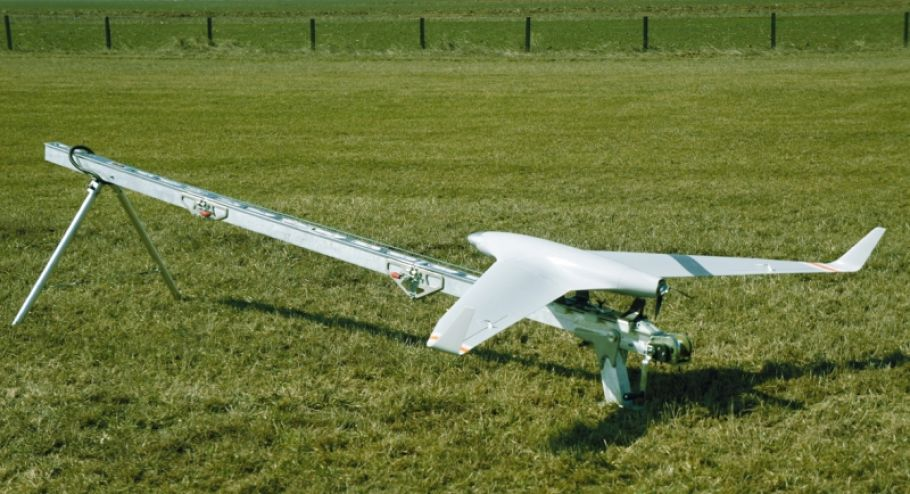
\includegraphics[width=3.5in]{img/hirrus.jpg}
\caption{Hirrus UAV [2]}
\textit{[2] http://aft.ro/bro.pdf}
\end{figure}
\end{center}
\end{frame}

\begin{frame}{Hirrus}

\begin{description}
\item [Destination] law enforcement, reconnaissance, search and rescue, cartography
\item [Dimensions] Wingspan 2.35 m / Length 1.1 m / Weight 7 kg
\item [Speed] Max 130 km/h, Cruise 90 km/h
\item [Payload] 0.7 kg
\item [Propulsion] Electric
\item [Endurance] 180 m
\item [Range] 15 km
\end{description}

\end{frame}

\begin{frame}{Platform Objectives}
\begin{itemize}
\item Ground Control System based on QGroundControl
\item Mission Monitor System
\item Remote Control Module for mission override and manual control
\item Autopilot for Hirrus with \textit{Collision Avoidance} and \textit{Formation
  Flight} modules
\item Artificial Intelligence Module for mission execution. 
\end{itemize}
\end{frame}

\begin{frame}{Platform Simulation Architecture}
\begin{center}
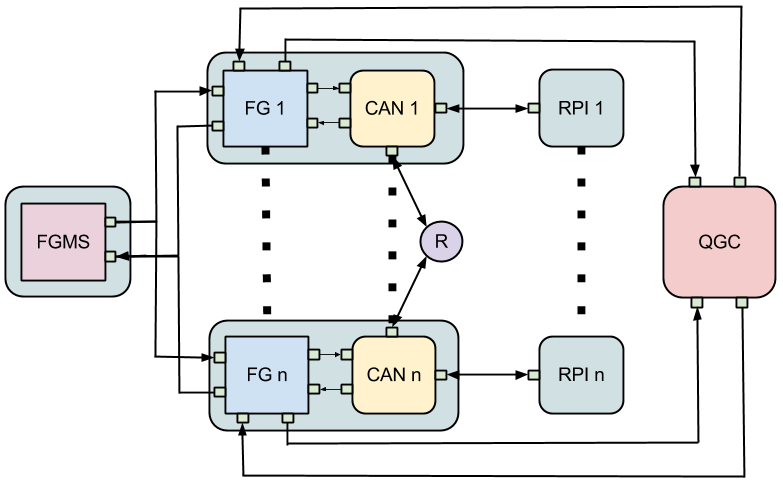
\includegraphics[width=3.5in]{img/platform-architecture.png}
\end{center}
\end{frame}
\begin{frame}{Autopilot Architecture}
\begin{center}
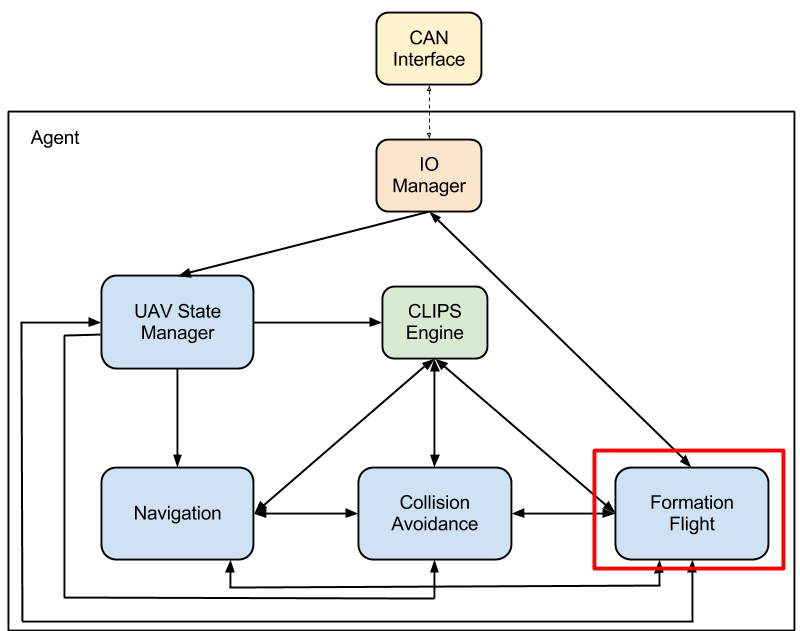
\includegraphics[width=3in]{img/rpi-architecture.png}
\end{center}
\end{frame}

\begin{frame}{Thesis Objectives}
\begin{itemize}
\item close range formation flight module
\item decentralized communication
\item reactive agents
\item inspired by real life animal swarms
\end{itemize}
\end{frame}

\begin{frame}{Formation Flight}
\begin{itemize}
\item 3 or more UAVs flying in formation
\item simulated using Flight Gear Flight Server
\item close range
\item follow the leader algorithm
\item GPS and ECEF coordinates based on WSG84 ellipsoid
\end{itemize}
\end{frame}

\begin{frame}{Types of Formation}
\begin{center}
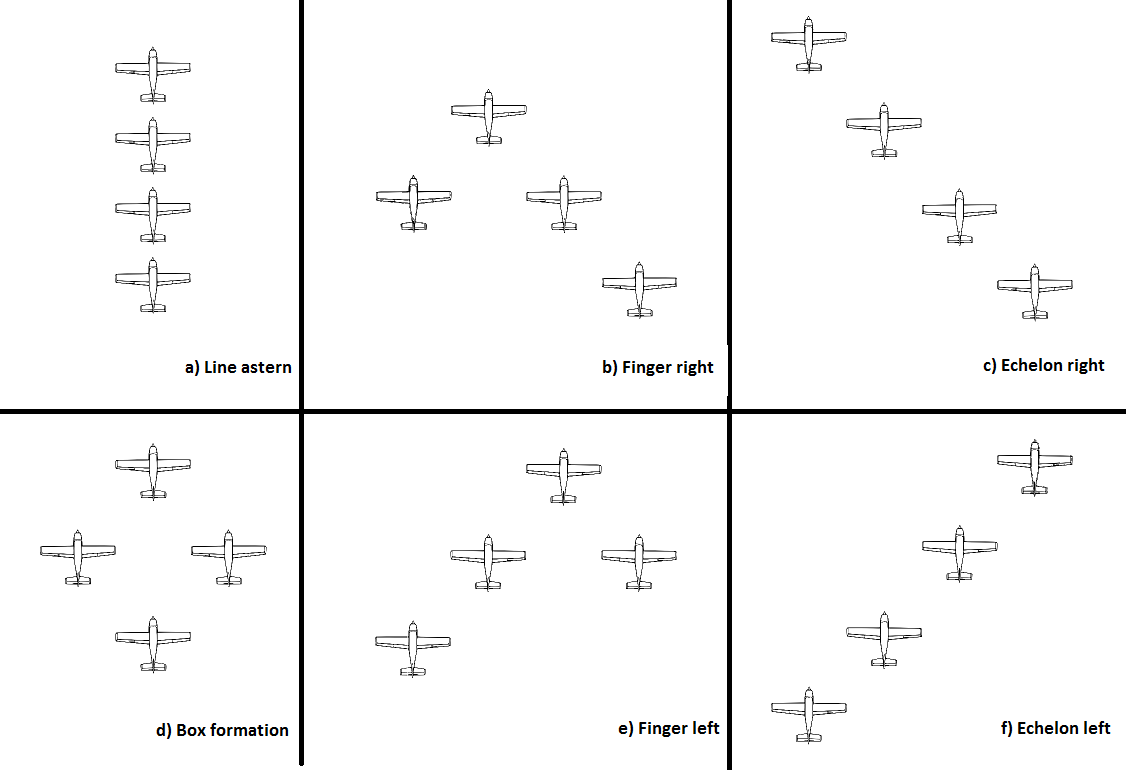
\includegraphics[width=1.7in]{img/4form.png}
\end{center}
\end{frame}

\begin{frame}{Tested Formations}

\begin{tabular}{l l}
\begin{minipage}{0.5\textwidth}
3 UAVs Formations
\begin{itemize}
\item{Line Astern}
\item{V Formation}
\end{itemize}\end{minipage}
&
\begin{minipage}{0.5\textwidth}
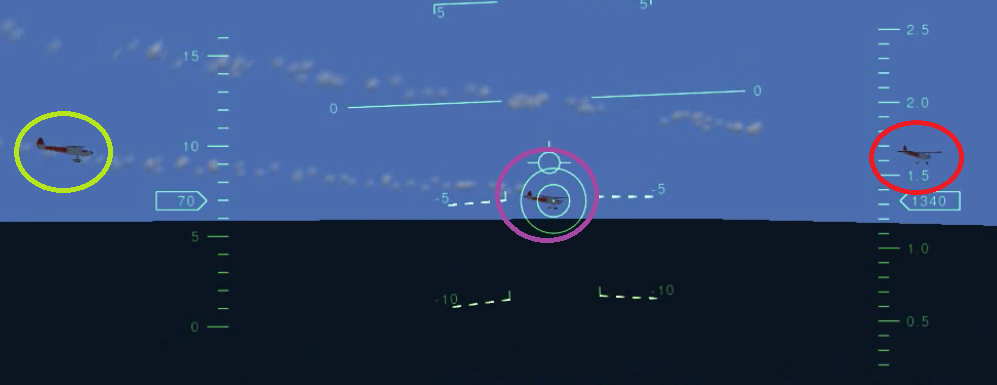
\includegraphics[width=2in]{img/line2.png}
\newline
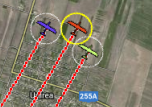
\includegraphics[width=2in]{img/vqgc.png}
\end{minipage}
\end{tabular}
\end{frame}

\begin{frame}{Evaluation and Results}
\begin{itemize}
\item tested with dedicated leader
\item leader with it's own mission
\item other UAVs have a \textit{follow the leader}
\item 9\% to 25\% of time spend for maintaining the formation
\item 60\% to 70\% of time spend for entering the formation
\item 15\% to 20\% of time relieving control for collision avoidance
\end{itemize}
\end{frame}

\begin{frame}{Evaluation and Results}
\begin{itemize}
\item communication delay can decrease the time spent in formation maintaining
\item communication delay can induce formation detachment
\item 300 feet ( $>$ 100 m) distance between UAVs
\item for tighter result another coordinate system is needed
\item computational errors are induced by the ellipsoid model while converting coordinates
\end{itemize}
\end{frame}

\begin{frame}{Evaluation and Results}
\begin{center}
\begin{figure}[p]
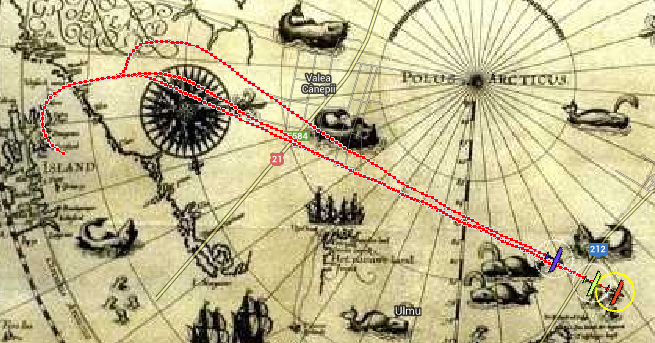
\includegraphics[width=4in]{img/lineastern.png}
% \caption{QGroundControl flight path for Line Astern simulation}
\end{figure}
\end{center}
\end{frame}

\begin{frame}{Future Work}
\begin{itemize}
\item formations based on a virtual leader (geometrical center of formation)
\item simulating with Flight Gear instances running on dedicated machines
\item communication between AI modules and Hirrus via CAN bus
\item PID controllers for speed and steering
\end{itemize}
\end{frame}

\begin{frame}{Questions}
\begin{center}
\fontsize{60}{70}\selectfont Q\&A
\end{center}
% Keywords:
% \begin{itemize}
% \item UAV
% \item Decentralized
% \item Reactive
% \item Flight Gear
% \item Hirrus
% \item QGroundControl
% \item Formations
% \item Communication
% \item Swarm
% \item Close Range Formation
% \end{itemize}
\end{frame}
\end{document}
